\documentclass[aspectratio=169,11pt]{beamer}
\usetheme{Madrid}
\usecolortheme{default}
\setbeamertemplate{navigation symbols}{}
\usepackage[utf8]{inputenc}
\usepackage[T1]{fontenc}
\usepackage[ngerman]{babel}
\usepackage{lmodern}
\usepackage{amsmath}
\usepackage{booktabs}
\usepackage{graphicx}
\usepackage{listings}
\usepackage{tikz}
\usetikzlibrary{arrows.meta,positioning,calc}
\hypersetup{pdftitle={Rangliste mit einem binaeren Suchbaum},pdfauthor={Projektteam},colorlinks=true,urlcolor=Teal}
\definecolor{Navy}{HTML}{14243B}
\definecolor{Teal}{HTML}{087F8C}
\definecolor{Amber}{HTML}{E9A23B}
\definecolor{Paper}{HTML}{F7F9FC}
\definecolor{Muted}{HTML}{526477}
\setbeamercolor{normal text}{fg=Navy,bg=white}
\setbeamercolor{structure}{fg=Teal}
\setbeamercolor{frametitle}{fg=Navy,bg=white}
\setbeamercolor{title}{fg=white,bg=Navy}
\setbeamercolor{block title}{fg=Teal,bg=Paper}
\setbeamercolor{block body}{fg=Navy,bg=Paper}
\setbeamertemplate{blocks}[default]
\setbeamertemplate{headline}{}
\setbeamerfont{frametitle}{size=\Large,series=\bfseries}
\setbeamerfont{title}{size=\LARGE,series=\bfseries}
\setbeamertemplate{frametitle}{\vspace{0.15cm}\insertframetitle\par\vspace{0.12cm}{\color{Teal}\rule{\textwidth}{0.6pt}}}
\setbeamertemplate{footline}{\leavevmode\hbox{\begin{beamercolorbox}[wd=.84\paperwidth,ht=2.6ex,dp=1.3ex,leftskip=.5cm]{normal text}\color{Muted}\tiny ADS -- Praktikum 05\end{beamercolorbox}\begin{beamercolorbox}[wd=.16\paperwidth,ht=2.6ex,dp=1.3ex,rightskip=.5cm plus1fil]{normal text}\hfill\color{Muted}\tiny\insertframenumber\end{beamercolorbox}}}
\setbeamersize{text margin left=0.65cm,text margin right=0.65cm}
\lstset{language=Java,basicstyle=\ttfamily\scriptsize,keywordstyle=\color{Teal}\bfseries,commentstyle=\color{Muted},stringstyle=\color{Teal},showstringspaces=false,columns=fullflexible,keepspaces=true,breaklines=true,backgroundcolor=\color{Paper},frame=none,xleftmargin=.12cm,xrightmargin=.12cm,aboveskip=.15cm,belowskip=.1cm}
\title{Rangliste mit einem\\binären Suchbaum}
\subtitle{Aufgabe 3 und ein Experiment zur Einfügereihenfolge}
\author{Name 1 \& Name 2}
\institute{ZHAW -- Algorithmen und Datenstrukturen}
\date{}
\begin{document}
% Messwerte stehen in results.tex. Diagramme stammen aus experiment/.
% Werte aus experiment/results/summary.json, Seed 20261019.
\newcommand{\ExperimentSeed}{20261019}
\newcommand{\ExactHeightMean}{5,017}
\newcommand{\MedianHeight}{14}
\newcommand{\OriginalHeight}{42}
\newcommand{\RandomComparisons}{42\,044}

\tikzset{treenode/.style={circle,draw=Teal,fill=Paper,line width=.7pt,minimum size=.58cm,inner sep=1pt,font=\small},treeedge/.style={draw=Muted,line width=.7pt}}

\begin{frame}[plain]
\begin{columns}[c,onlytextwidth]
\column{.66\textwidth}
{\color{Teal}\small ALGORITHMEN UND DATENSTRUKTUREN}\par\vspace{.35cm}
{\color{Navy}\fontsize{27}{32}\selectfont\bfseries Rangliste mit einem\\binären Suchbaum}\par\vspace{.35cm}
{\large Aufgabe 3: Implementierung und Experiment}\par\vspace{.75cm}
{\color{Muted}\small \insertauthor\\\insertinstitute}\par
\column{.30\textwidth}
\centering
{\color{Teal}\fontsize{42}{46}\selectfont\bfseries 3\,166}\par
\small Teilnehmer aus der CSV\par\vspace{.65cm}
\raggedright
\normalsize Wie stark verändert die\newline Einfügereihenfolge\newline den Aufwand?
\end{columns}
\note{Person 1, ca. 25 Sekunden. Wir lösen Aufgabe 3: Aus einer Teilnehmerdatei soll eine Rangliste entstehen. Dazu verwenden wir einen normalen binären Suchbaum. Anschliessend untersuchen wir, wie stark die Reihenfolge beim Einfügen die Baumform und den Aufwand verändert.}
\end{frame}

\begin{frame}{Suchbaum und sortierte Ausgabe}
\begin{columns}[c,onlytextwidth]
\column{.55\textwidth}
\centering
\begin{tikzpicture}[x=1cm,y=1cm]
\node[treenode,minimum size=1.0cm] (r) at (0,0) {2:30};
\node[treenode,minimum size=1.0cm] (l) at (-1.6,-1.15) {2:20};
\node[treenode,minimum size=1.0cm] (rr) at (1.6,-1.15) {2:40};
\node[treenode,minimum size=1.0cm] (ll) at (-2.5,-2.35) {2:10};
\node[treenode,minimum size=1.0cm] (lr) at (-.7,-2.35) {2:25};
\draw[treeedge] (r)--(l) (r)--(rr) (l)--(ll) (l)--(lr);
\node[font=\small,text=Teal] at (-1.55,.6) {links $\leq$};
\node[font=\small,text=Teal] at (1.6,.6) {rechts $>$};
\node[font=\scriptsize,text=Muted] at (-.4,-3.05) {Beispielzeiten in Stunden:Minuten};
\end{tikzpicture}
\column{.41\textwidth}
\textbf{Ordnung im Baum}\par\medskip
\texttt{compareTo()} vergleicht die Laufzeiten. Gleiche Zeiten gehen nach links.
\par\vspace{.55cm}
\textbf{Inorder}\par\medskip
Links, Knoten, rechts\par\medskip
{\color{Teal}\large 2:10, 2:20, 2:25, 2:30, 2:40}
\end{columns}
\note{Person 1, ca. 50 Sekunden. Jeder Knoten enthält einen Teilnehmer. Links liegen kleinere oder gleiche Laufzeiten, rechts grössere. Das gilt in jedem Teilbaum. Inorder besucht erst links, dann den aktuellen Knoten und dann rechts. Dadurch erhalten wir die Teilnehmer nach Laufzeit. Der Baum ist geordnet, aber noch nicht automatisch ausgeglichen. Die Zeiten in dieser Zeichnung sind nur ein Beispiel.}
\end{frame}

\begin{frame}[fragile]{Implementierung: Einfügen und Visitor}
\begin{columns}[T,onlytextwidth]
\column{.48\textwidth}
\textbf{1. Teilnehmer einfügen}\par\smallskip
\begin{lstlisting}
Tree<Competitor> tree =
    new SortedBinaryTree<>();

// Je gueltiger CSV-Zeile:
tree.add(new Competitor(
    0, name, time));
\end{lstlisting}
\small\texttt{createTree()} zerlegt die Zeilen, prüft das Format und füllt den Baum.
\column{.48\textwidth}
\textbf{2. Rang und Text erzeugen}\par\smallskip
\begin{lstlisting}
AtomicInteger rank =
    new AtomicInteger(1);
StringBuilder sb = new StringBuilder();

tree.traversal().inorder(c -> {
    c.setRank(rank.getAndIncrement());
    sb.append(c).append("\n");
});
\end{lstlisting}
\end{columns}
\vspace{.45cm}
{\color{Teal}\textbf{Traversierung: Reihenfolge. \quad Visitor: Aktion je Teilnehmer.}}
\par\smallskip\scriptsize Ausschnitte aus \texttt{RankingTreeServer}; Ränge 1, 2, 3, \ldots\ auch bei Zeitgleichheit.
\note{Person 1, ca. 65 Sekunden. Links sehen wir den Kern von createTree. Die vollständige Methode behandelt auch Leerzeilen und Windows-Zeilenumbrüche und kontrolliert Name und Zeitformat. Die add-Methode entscheidet mit compareTo, ob sie links oder rechts weitersucht. Rechts erzeugen wir die Ausgabe. Das Lambda implementiert die einzige Visitor-Methode visit. Bei jedem Teilnehmer setzen wir einen Rang und hängen eine Zeile an. AtomicInteger ermöglicht einen veränderlichen Zähler innerhalb des Lambdas. Das hat hier nichts mit paralleler Ausführung zu tun. Die Rangnummern steigen gemäss Vorlage fortlaufend, auch bei gleicher Zeit.}
\end{frame}

\begin{frame}{Laufzeit von Aufbau und Ausgabe}
\vspace{.1cm}
\centering
\renewcommand{\arraystretch}{1.5}
\begin{tabular}{@{}lccc@{}}
\toprule
 & \textbf{Best Case} & \textbf{Average Case$^*$} & \textbf{Worst Case}\\
\midrule
Baumhöhe $h$ & $\Theta(\log n)$ & erwartet $\Theta(\log n)$ & $\Theta(n)$\\
Aufbau & $\Theta(n\log n)$ & erwartet $\Theta(n\log n)$ & $\Theta(n^2)$\\
Inorder-Ausgabe & $\Theta(n)$ & $\Theta(n)$ & $\Theta(n)$\\
\bottomrule
\end{tabular}
\par\vspace{.25cm}
\raggedright
\textbf{Worst Case bei acht Werten:}\quad $0+1+2+3+4+5+6+7=\mathbf{28}$
\par\smallskip
\[
 C_{\mathrm{worst}}(n)=\frac{n(n-1)}{2}
 =\frac{1}{2}n^2-\frac{1}{2}n
 \quad\Longrightarrow\quad \color{Teal}\boxed{\Theta(n^2)}
\]
\vspace{-.15cm}
\small\textcolor{Teal}{\textbf{Die Laufzeitklasse beschreibt das Wachstum.}}\quad Exakte Anzahl bei $n=8$: 28.
\par\smallskip
\scriptsize Einfügen: $O(h)$. Gesamtaufwand: Aufbau + Inorder. Speicher: $\Theta(n)$ und $O(h)$ Rekursionsstack.
\par\vspace{.18cm}
\raggedright\tiny $^*$Klassische Erwartung für verschiedene Schlüssel in gleichverteilt zufälliger Reihenfolge. CSV-Zeitgleichheiten untersuchen wir empirisch. Konstant grosse Zeitfelder; Ausgabetext linear in seiner Länge. Theorie: Sedgewick/Wayne, \href{https://algs4.cs.princeton.edu/32bst/}{Binary Search Trees}.
\note{Person 1, ca. 65 Sekunden. Ein einzelnes Einfügen folgt einem Pfad und kostet O von h. In einem flachen Baum ergibt der gesamte Aufbau n log n. Im schlechtesten Fall entsteht eine Kette: Die erste Einfügung braucht null Vergleiche, die zweite einen, die letzte bei acht Werten sieben. Zusammen sind das 28. Allgemein ist die Summe n mal n minus eins durch zwei, also ein halbes n Quadrat minus ein halbes n. Für die Laufzeitklasse zählt das dominierende quadratische Wachstum. Deshalb steht hier Theta von n Quadrat, obwohl die genaue Vergleichszahl bei acht Werten 28 beträgt und nicht 64. Inorder besucht danach immer jeden Teilnehmer genau einmal. Der klassische Average Case setzt verschiedene Schlüssel in zufälliger Reihenfolge voraus. Übergabe an Person 2.}
\end{frame}

\begin{frame}{Experiment: vollständig und als Stichprobe}
\begin{columns}[T,onlytextwidth]
\column{.47\textwidth}
{\color{Teal}\fontsize{29}{32}\selectfont\bfseries 40\,320}\par\smallskip
\textbf{Alle $8!$ Reihenfolgen}\par\medskip
\small Acht verschiedene Zeiten, über die sortierten CSV-Zeiten verteilt. Wir untersuchen jede ihrer Permutationen.
\column{.47\textwidth}
{\color{Teal}\fontsize{29}{32}\selectfont\bfseries 10\,000}\par\smallskip
\textbf{Zufallsreihenfolgen der ganzen CSV}\par\medskip
\small Je 3\,166 Teilnehmer, fester Seed. Dazu Originaldatei, Median zuerst und sortierte Reihenfolgen.
\end{columns}
\vspace{.55cm}
\textbf{Messgrössen:}\quad Höhe in Ebenen und Vergleiche beim Einfügen.
\par\medskip
\small Alle Reihenfolgen der 3\,166 markierten Datensätze wären rund $10^{9710}$. Eine vollständige Untersuchung ist damit praktisch unmöglich.
\par\vspace{.35cm}
\tiny Messmodell: dieselbe Einfügeregel mit vorberechneten Sekundenwerten, gegen den Java-Baum geprüft. Keine Zeitmessung in Millisekunden. 2\,459 verschiedene Zeiten; doppelte Werte bleiben erhalten. Seed: \ExperimentSeed.
\note{Person 2, ca. 55 Sekunden. Wir erweitern die Idee aus Aufgabe 4: Für jede Einfügereihenfolge bauen wir einen neuen Baum und messen seine Höhe. Zusätzlich zählen wir die Schlüsselvergleiche. Für acht unterschiedliche Zeiten schaffen wir wirklich alle 40320 Reihenfolgen. Für die ganze Datei ist das unmöglich, denn die Zahl der Permutationen hat etwa 9710 Dezimalstellen. Hier verwenden wir 10000 pseudorandom gleichverteilt erzeugte Permutationen mit festem Seed. Das Modell verwendet die gleichen Vergleichsergebnisse und die gleiche Links-rechts-Regel wie unser Java-Code, aber vorberechnete Sekundenwerte. Deshalb messen wir algorithmische Arbeit, keine Ausführungszeit. Identische Zeilen ändern die enorme Grössenordnung der Permutationszahl nicht.}
\end{frame}

\begin{frame}{Acht Teilnehmer: die vollständige Verteilung}
\centering
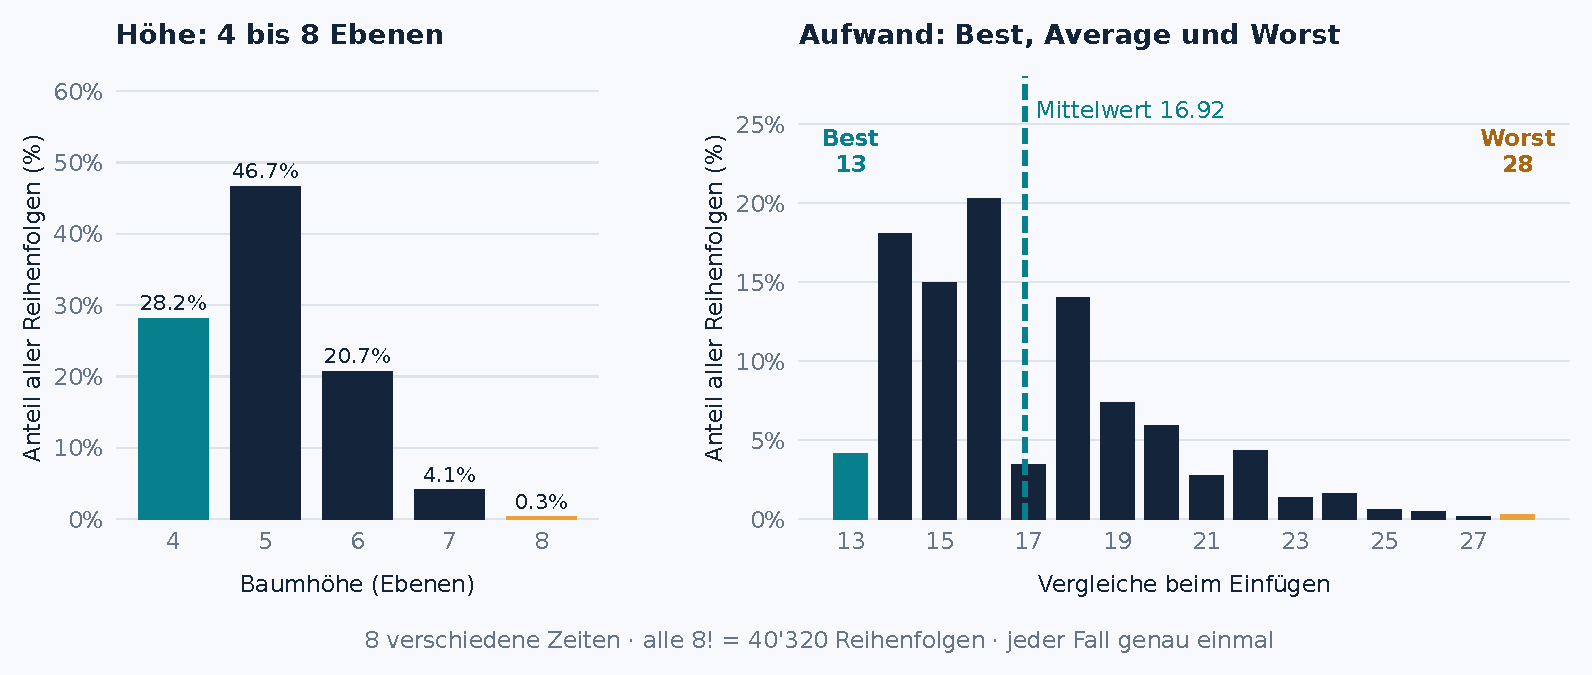
\includegraphics[width=.96\textwidth,height=4.9cm,keepaspectratio]{images/exhaustive_heights.pdf}
\par\vspace{.1cm}
\begin{columns}[T,onlytextwidth]
\column{.54\textwidth}
\small\textcolor{Teal}{\textbf{Best Case: kurze Einfügewege}}\par\smallskip
$0+1+1+2+2+2+2+3=\mathbf{13}$
\column{.42\textwidth}
\small\textcolor{Amber}{\textbf{Worst Case: eine Kette}}\par\smallskip
$0+1+\cdots+7=\mathbf{28}$\par\smallskip
\scriptsize Wachstum für grösseres $n$: $\Theta(n^2)$.
\end{columns}
\note{Person 2, ca. 60 Sekunden. Links zeigt die Grafik die Baumhöhen, rechts die Anzahl der Einfügevergleiche. Jede Zahl in den Summen unten steht für die Vergleiche einer einzelnen Einfügung. Im besten Fall braucht die Wurzel null, ihre zwei Kinder je einen und die vier Knoten der nächsten Ebene je zwei Vergleiche. Der achte Knoten liegt eine Ebene tiefer und braucht drei. Das ergibt 13. Im Worst Case entsteht eine Kette mit null bis sieben Vergleichen, insgesamt 28. Wie auf der Laufzeitfolie erklärt, wächst diese Summe quadratisch. Der Mittelwert über alle 40320 Reihenfolgen beträgt exakt 682272 geteilt durch 40320, gerundet 16,92. Weil jede Reihenfolge enthalten ist, sind das genaue Ergebnisse und keine Stichprobenschätzungen.}
\end{frame}

\begin{frame}{Die ganze CSV: Höhe und Einfügeaufwand}
\centering
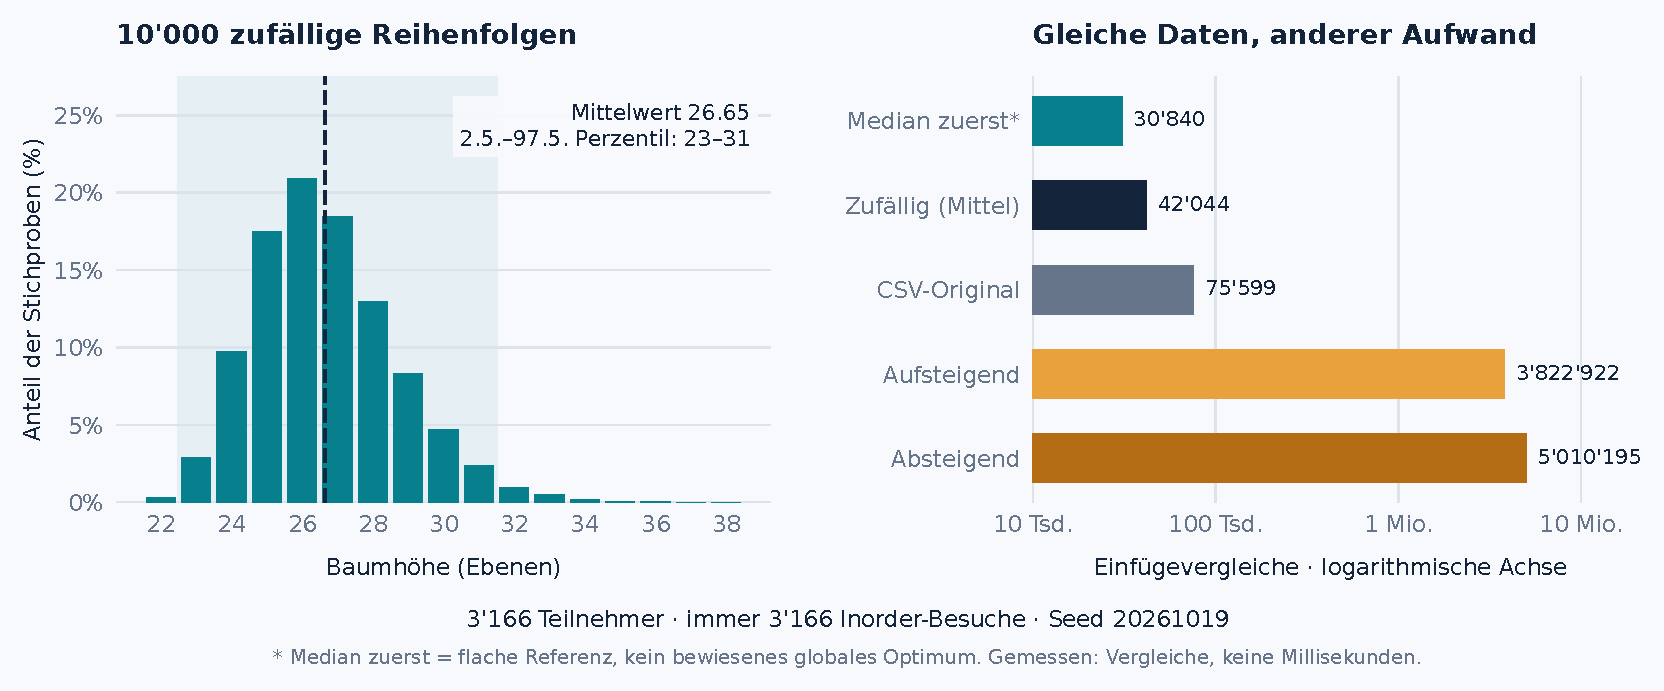
\includegraphics[width=.99\textwidth,height=5.25cm,keepaspectratio]{images/full_csv_main.pdf}
\par\vspace{.1cm}
\small Höhe: Median zuerst \textbf{14}, Originaldatei \textbf{42}, absteigend \textbf{3\,166}.
\note{Person 2, ca. 55 Sekunden. Links zeigen die Balken die 10000 vollständigen Zufallsreihenfolgen. Mittelwert und Quantile beziehen sich nur auf diese Stichprobe. Rechts vergleichen wir den Aufwand auf einer logarithmischen Achse. Zufällig benötigen wir im Mittel rund 42044 Vergleiche, absteigend gut fünf Millionen, also etwa 119-mal so viele. Absteigende Eingabe erzeugt auch mit gleichen Zeiten eine linke Kette. Dann ist die Vergleichszahl exakt n mal n minus eins geteilt durch zwei. Der flache Medianfall ist eine Referenz, aber wegen der Duplikate behaupten wir für diese konkrete CSV kein bewiesenes globales Optimum. Aufsteigende Zeiten bilden wegen der links eingefügten Duplikate keine reine Kette.}
\end{frame}

\begin{frame}{Warum diese Fälle entstehen}
\begin{columns}[T,onlytextwidth]
\column{.31\textwidth}
\centering\textcolor{Teal}{\textbf{Flacher Baum}}\par\smallskip
\begin{minipage}[c][2.9cm][c]{\linewidth}\centering
\begin{tikzpicture}[scale=.7]
\foreach \id/\x/\y/\txt in {a/0/0/4,b/-1.2/-1/2,c/1.2/-1/6,d/-1.8/-2/1,e/-.6/-2/3,f/.6/-2/5,g/1.8/-2/7}{\node[treenode] (\id) at (\x,\y) {\txt};}
\draw[treeedge] (a)--(b) (a)--(c) (b)--(d) (b)--(e) (c)--(f) (c)--(g);
\end{tikzpicture}
\end{minipage}
\par\small Mittlere Schlüssel zuerst teilen die Werte auf beide Seiten auf.
\column{.31\textwidth}
\centering\textbf{Zufällige Reihenfolge}\par\smallskip
\begin{minipage}[c][2.9cm][c]{\linewidth}\centering
\begin{tikzpicture}[scale=.7]
\foreach \id/\x/\y/\txt in {a/0/0/3,b/-1/-1/1,c/1/-1/6,d/-.3/-2/2,e/.5/-2/5,f/1.8/-2/7,g/-.1/-3/4}{\node[treenode] (\id) at (\x,\y) {\txt};}
\draw[treeedge] (a)--(b) (a)--(c) (b)--(d) (c)--(e) (c)--(f) (e)--(g);
\end{tikzpicture}
\end{minipage}
\par\small Unterschiedliche Teilungen ergeben eine Streuung der Höhen.
\column{.31\textwidth}
\centering\textcolor{Amber}{\textbf{Absteigende Reihenfolge}}\par\smallskip
\begin{minipage}[c][2.9cm][c]{\linewidth}\centering
\begin{tikzpicture}[scale=.8]
\foreach \i in {0,...,6}{\pgfmathtruncatemacro{\txt}{7-\i}\node[treenode,draw=Amber,minimum size=.42cm,font=\scriptsize] (n\i) at (-.5*\i,-.5*\i) {\txt};}
\foreach \i in {1,...,6}{\pgfmathtruncatemacro{\prev}{\i-1}\draw[treeedge] (n\prev)--(n\i);}
\end{tikzpicture}
\end{minipage}
\par\small Jeder neue Wert folgt demselben Ast. Es entsteht eine Kette.
\end{columns}
\vspace{.35cm}
\textcolor{Teal}{\textbf{Die Einfügereihenfolge bestimmt die Baumform und damit den Aufwand.}}
\par\smallskip\scriptsize Beispiele mit sieben unterschiedlichen Schlüsseln. Ein AVL- oder Rot-Schwarz-Baum würde seine Höhe selbst begrenzen.
\note{Person 2, ca. 45 Sekunden. Links sehen wir das Prinzip des Best Case: Mittlere Schlüssel zuerst erzeugen kurze Wege. Die zufällige Reihenfolge erzeugt viele verschiedene Formen, meist ohne vollständige Entartung. Absteigend landet jeder neue Wert links, sodass die Pfade immer länger werden. Daher entstehen 0 plus 1 plus 2 bis n minus 1 Vergleiche und quadratischer Aufwand. Unsere Rangliste ist in allen Fällen korrekt sortiert, aber der Aufwand unterscheidet sich stark. Die Methode balanced prüft nur, sie gleicht nichts aus. Eine selbstbalancierende Datenstruktur wäre die mögliche Weiterentwicklung.}
\end{frame}

\end{document}
